\section{Pianificazione}
In questa sezione verrà riportata come l'attività di pianificazione del progetto è stata gestita dal gruppo Catch Em All. Il gruppo ha deciso di suddividere questa attività in vari periodi: 
\begin{itemize}
	\item \textbf{Analisi};
	\item \textbf{Sviluppo del Proof of Concept};
	\item \textbf{Progettazione architetturale};
    \item \textbf{Progettazione di dettaglio e Codifica};
	\item \textbf{Validazione\textsubscript{G} e Collaudo}.
\end{itemize}

\subsection{Analisi}
\subsubsection{Scopo}
Questo periodo ha lo scopo di analizzare in dettaglio il capitolato scelto dal gruppo in modo da definire i requisiti\textsubscript{G} funzionali, tempi e costi del progetto e gli obiettivi di qualità. Vengono anche definite in questo periodo le varie norme che il gruppo dovrà seguire per lavorare in modo efficacie ed efficiente.

\subsubsection{Periodo}
Il periodo di analisi inizierà con l'aggiudicazione del capitolato il 07/11/2022 e si svolgerà fino al completamento dei vari documenti necessari alla revisione  RTB. Il gruppo ha pianificato la fine di questo periodo per il 12/02/2023. Questo periodo sarà a sua volta suddiviso in vari sprint per ripartire in modo organizzato le attività che lo compongono.

\subsubsection{Ruoli attivi}
Durante il periodo di analisi saranno necessari i seguenti ruoli:
\begin{itemize}
	\item Responsabile;
	\item Amministratore;
	\item Analista;
	\item Verificatore.
\end{itemize}

\subsubsection{Sprint I}
\subsubsubsection{Scopo}
Lo scopo del primo sprint è quello di compiere una prima analisi del capitolato e impostare le prime norme e strumenti necessari che faranno da base al way of working del gruppo. Vengono inoltre redatti i primi verbali in modo da tenere traccia delle decisioni prese negli incontri interni e con il proponente.
\subsubsubsection{Durata}
Questo sprint si svolgerà nelle prime settimane di progetto. Inizierà il 07/11/2022 e terminerà il 27/11/2022.

\subsubsubsection{Precondizioni}\:
\begin{itemize}
	\item È stato formato il gruppo Catch Em All;
	\item È stato assegnato il capitolato d’appalto C1: \textit{CAPTCHA: umano o sovrumano?}.
\end{itemize}

\subsubsubsection{Postcondizioni}\:
\begin{itemize}
	\item Compiuta analisi preliminare del capitolato, seguita da uno studio di fattibilità sulle idee proposte dal gruppo;
	\item Scelti strumenti per la gestione dei compiti e ruoli dei vari membri;
	\item Scelta strumenti per la stesura dei documenti;
	\item Scrittura bozza dei documenti necessari alla revisione RTB;
	\item Fissata una base per il way of working del gruppo.
\end{itemize}

\subsubsubsection{Attività}\:
\begin{itemize}
	\item \textbf{Analisi preliminare fattibilità del capitolato}: Vengono discusse le varie proposte del gruppo per lo sviluppo del progetto, analizzandone pro e contro;
	\item \textbf{Ricerca degli strumenti}: Individuazione degli strumenti organizzativi e di supporto che saranno utilizzati durante il progetto per la suddivisione dei compiti e scrittura dei documenti;
	\item \textbf{Normazione}: Definizione delle norme alla base del way of working del gruppo, le quali sono illustrate nel documento \textit{Norme\_di\_progetto v 1.0.0};
    \item \textbf{Analisi dei requisiti}: Attività finalizzata alla comprensione dei bisogni espressi nel capitolato d’appalto e ricavati dallo studio del dominio\textsubscript{G} d’uso;
    \item \textbf{Analisi dei rischi}: Compiere una prima analisi dei rischi che il gruppo potrà incontrare nello sviluppo del progetto e fornire delle contromisure per evitare o ammortizzare i danni che questi possono causare.
\end{itemize}
\newpage
\subsubsection{Sprint II}\:
\subsubsubsection{Scopo}
Lo scopo del secondo sprint è quello di continuare l'analisi dei requisiti e dei casi d'uso del progetto, decidendo anche quali siano gli obiettivi di qualità che il progetto dovrà soddisfare. Vengono inoltre compiute una pianificazione e preventivo più dettagliate per la durata e i costi del progetto. In questo sprint il way of working del gruppo verrà migliorato in base ai riscontri ottenuti nel corso dello sprint precedente per avere un continuo miglioramento di efficienza ed efficacia nella completamento dei vari compiti assegnati ai membri.
\subsubsubsection{Durata}
Questo sprint seguirà le fasi iniziali del progetto. Inizierà il 28/11/2022 e terminerà il 25/12/2022.

\subsubsubsection{Precondizioni}\:
\begin{itemize}
	\item È stata svolta un analisi preliminare del capitolato;
	\item È stata impostata una base solida per il way of working del gruppo.
\end{itemize}

\subsubsubsection{Postcondizioni}\:
\begin{itemize}
	\item Definiti requisiti e casi d'uso necessari per il progetto, accompagnati dai vari obiettivi di qualità che dovranno essere rispettati;
	\item Pianificazione periodi e attività per l'intera durata del progetto;
	\item Fissate le varie norme che comporranno il way of working del gruppo.
\end{itemize}

\subsubsubsection{Attività}\:
\begin{itemize}
	\item \textbf{Normazione}: Definizione delle varie norme per i processi organizzativi e di supporto.
	\item \textbf{Obiettivi e metriche di qualità}: Individuazione degli obiettivi e metriche necessarie a garantire la qualità dei processi e dei prodotti per l'intera durata del progetto;
	\item \textbf{Analisi dei requisiti e casi d'uso}: Ricerca di tutti i requisiti e casi d'uso necessari per lo sviluppo del progetto;
	\item \textbf{Pianificazione periodi e attività}: Strutturare la pianificazione dei vari periodi del progetto fissando attività e obiettivi da raggiungere.
\end{itemize}

\subsubsection{Sprint III}
\subsubsubsection{Scopo}
Lo scopo del terzo sprint è quello di compiere una prima verifica completa delle attività svolte, e di conseguenza verificare che i vari documenti prodotti rispettino le norme definite e che i loro contenuti siano adeguati. In questo sprint viene inoltre svolta un'analisi sul way of working del gruppo, su come sia possibile migliorarlo e di come siano stati affrontati i vari imprevisti incontrati.
\subsubsubsection{Durata}
Questo sprint si svolgerà dopo la conclusione dell'analisi completa dei requisiti e casi d'uso del progetto e di una buona pianificazione di esso. Inizierà il 26/12/2022 e terminerà il 09/01/2023.

\subsubsubsection{Precondizioni}\:
\begin{itemize}
	\item È stato completata l'analisi dei requisiti e casi d'uso del progetto;
	\item I vari periodi e attività del progetto sono state definite.
\end{itemize}

\subsubsubsection{Postcondizioni}\:
\begin{itemize}
	\item Verifica della struttura e contenuti dei documenti prodotti;
	\item Compiuta analisi per il miglioramento del way of working sulle attività svolte.
\end{itemize}

\subsubsubsection{Attività}\:
\begin{itemize}
	\item \textbf{Normazione}: Aggiornamento delle norme in base ai riscontri e analisi svolte su attività completate;
	\item \textbf{Verifica}: Controllo qualità della struttura e contenuti dei documenti prodotti.
\end{itemize}

\subsubsection{Sprint V}
\subsubsubsection{Scopo}
Questo sprint è condiviso al periodo di \textit{Produzione del Proof of Concept}.
Lo scopo del quinto sprint per il periodo di \textit{Analisi} è quello di aggiornare i requisiti e casi d'uso del progetto a seguito dei riscontri ottenuti nelle attività di sviluppo del PoC.
\subsubsubsection{Durata}
Questo sprint si svolgerà parallelamente alle attività di sviluppo del PoC. Inizierà il 30/01/2023 e terminerà il 12/02/2023.

\subsubsubsection{Precondizioni}\:
\begin{itemize}
	\item È stata completata un'analisi delle tecnologie e della struttura del PoC;
	\item È stata impostata una base solida per lo sviluppo PoC.
\end{itemize}

\subsubsubsection{Postcondizioni}\:
\begin{itemize}
	\item Definiti in modo completo requisiti e casi d'uso del progetto;
	\item Definiti in modo chiaro obiettivi di qualità e test del sistema.
\end{itemize}

\subsubsubsection{Attività}\:
\begin{itemize}
	\item \textbf{Aggiornamento requisiti e casi d'uso}: Aggiornamento dei requisiti e casi d'uso in base ai riscontri ottenuti dallo sviluppo del PoC;
	\item \textbf{Miglioramento obiettivi di qualità}: Revisione e miglioramento degli obiettivi e metriche di qualità definite;
	\item \textbf{Test di sistema}: Definizione dei test di sistema che dovranno essere svolti sul prodotto finale.
\end{itemize}

\subsubsection{Diagramma di Gantt\textsubscript{G} - Analisi}

\begin{figure}[H]
\centering
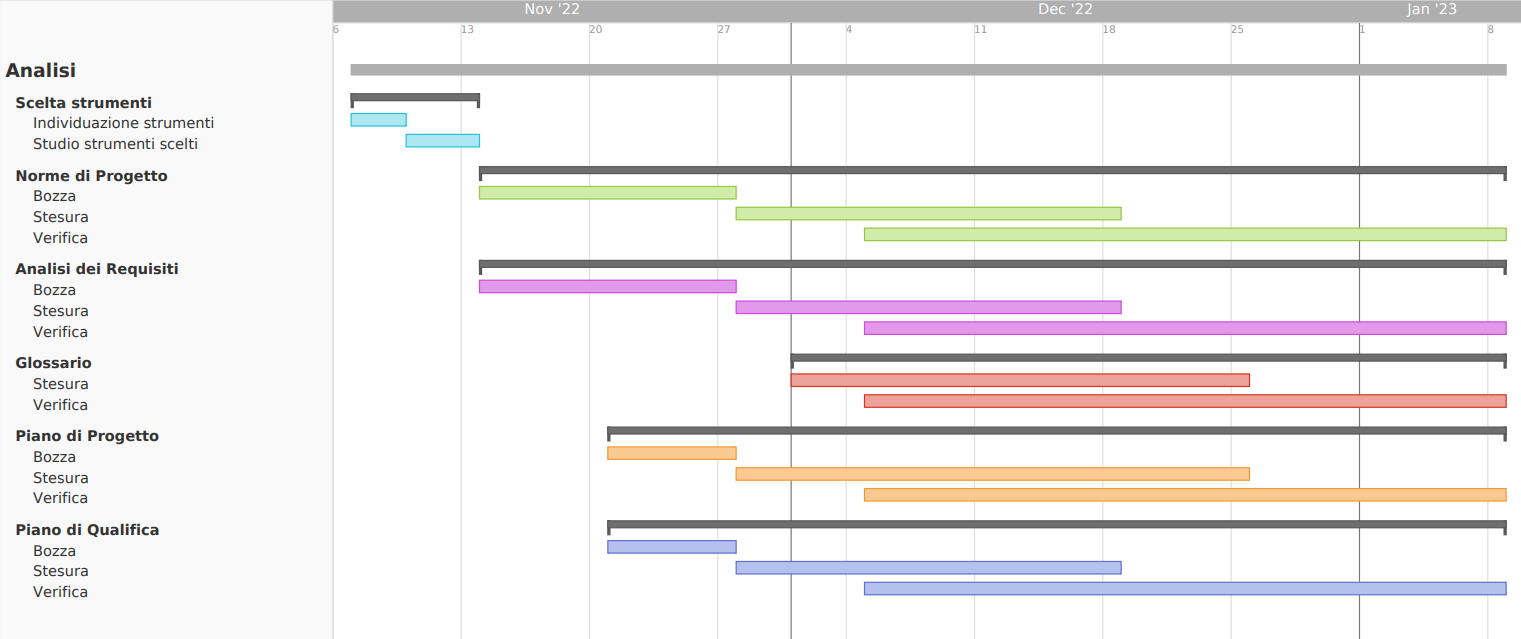
\includegraphics[width=\textwidth]{img/4_analisi.png}
\caption{Analisi}
\end{figure}

\subsection{Produzione del Proof of Concept}
\subsubsection{Scopo}
Gli obiettivi di questa fase sono lo studio delle possibili soluzioni architetturali per il \textit{PoC\textsubscript{G}} e l’individuazione dell’architettura di base per l’implementazione del prodotto. Segue a ciò l’attività di codifica del \textit{PoC\textsubscript{G}}.\\
La fase di produzione del Proof of Concept terminerà con la prima revisione \textit{RTB}.

\subsubsection{Periodo}
La fase di  si svolgerà dal  fino al 24/02/2023.
Il periodo di produzione del Proof of Concept inizierà dopo che il gruppo avrà svolto una solida analisi dei requisiti e l'inizio è pianificato per il 09/01/2023 e si svolgerà fino alla prima revisione di RTB, pianificata per 24/02/2023.

\subsubsection{Ruoli attivi}
Durante la fase di produzione del Proof of Concept lisi saranno necessari i seguenti ruoli:
\begin{itemize}
	\item Responsabile;
    \item Amministratore;
    \item Analista;
    \item Progettista;
    \item Programmatore;
    \item Verificatore.
\end{itemize}

\subsubsection{Sprint IV}
\subsubsubsection{Scopo}
Lo scopo di questo sprint è quello di iniziare la realizzazione del Proof of Concept, iniziando con la scelta delle tecnologie da utilizzare e seguito da uno studio approfondito su di essi.
\subsubsubsection{Durata}
Questo sprint avrà durata di tre settimane. Inizierà il 09/01/2023 e terminerà il 29/01/2023.

\subsubsubsection{Precondizioni}
I seguenti documenti sono stati redatti:
\begin{itemize}
	\item Norme di Progetto;
	\item Analisi dei Requisiti;
	\item Glossario;
    \item Piano di Progetto;
	\item Piano di Qualifica.
\end{itemize}

\subsubsubsection{Postcondizioni}\:
\begin{itemize}
	\item Aggiornamento e miglioramento dei documenti in precedenza redatti durante la fase di Analisi;
	\item Determinate le tecnologie da utilizzare;
	\item I membri del gruppo hanno acquisito conoscenze sull'uso delle tecnologie scelte;
	\item Pronto per la parte di codifica del \textit{PoC\textsubscript{G}}.
\end{itemize}

\subsubsubsection{Attività}\:
\begin{itemize}
	\item \textbf{Aggiornamento e miglioramento dei documenti}: Attività finalizzata a migliorare, se necessario, i documenti prodotti nella fase precedente aggiungendo nuovi elementi;
	\item \textbf{Individuazione requisiti\textsubscript{G} per il \textit{PoC\textsubscript{G}}}: Attività di analisi finalizzata all’individuazione dei requisiti\textsubscript{G} che il \textit{PoC\textsubscript{G}} andrà a soddisfare;
    \item \textbf{Progettazione Technology Baseline\textsubscript{G}}: Individuazione dell’architettura di base per l’implementazione del prodotto;
        \subitem \textbf{Approfondimento sulle tecnologie scelte}: I membri del gruppo si dedicano allo studio individuale delle tecnologie selezionate; al termine di questa attività tutti avranno acquisito le competenze necessarie per poter lavorare a rotazione sulla produzione del \textit{PoC\textsubscript{G}};
\end{itemize}

\subsubsection{Sprint V}
\subsubsubsection{Scopo}
Questo sprint è condiviso al periodo di \textit{Analisi}. Lo scopo di questo sprint è la realizzazione effettiva del \textit{PoC\textsubscript{G}} utilizzando le tecnologie scelte nello scorso sprint.
\subsubsubsection{Durata}
Questo sprint avrà durata di due settimane. Inizierà il 30/01/2023 e terminerà il 12/02/2023.

\subsubsubsection{Precondizioni}\:
\begin{itemize}
	\item Sono state determinate tecnologie da utilizzare per la realizzazione del \textit{PoC\textsubscript{G}};
	\item E' stato fatto uno studio approfondito sulle tecnologie scelte.
\end{itemize}

\subsubsubsection{Postcondizioni}\:
\begin{itemize}
	\item E' stato sviluppato il \textit{PoC\textsubscript{G}};
	\item Pronto per la verifica e controlli.
\end{itemize}

\subsubsubsection{Attività}\:
\begin{itemize}
    \item \textbf{Sviluppo della Technology Baseline\textsubscript{G}}: Attività di codifica del \textit{PoC\textsubscript{G}};
\end{itemize}

\subsubsection{Diagramma di Gantt\textsubscript{G} - Produzione del Proof of Concept}

\begin{figure}[H]
\centering
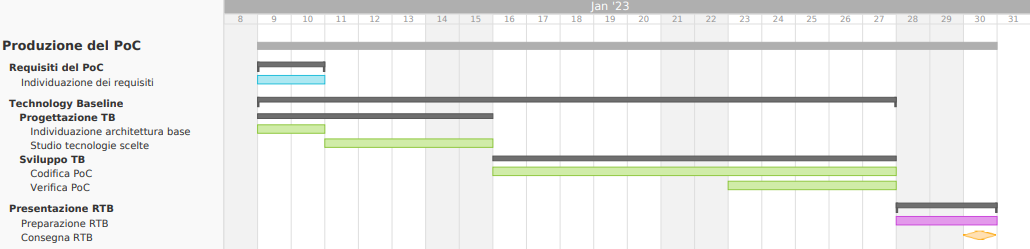
\includegraphics[width=\textwidth]{img/4_produzione.png}
\caption{Produzione del Proof of Concept}
\end{figure}

\subsection{Progettazione architetturale}
Lo scopo di questa fase è il raffinamento della progettazione architetturale ad alto livello avviata nella fase descritta al paragrafo \textit{4.2 Produzione del Proof of Concept}, ovvero “come” saranno soddisfatti i requisiti\textsubscript{G} precedentemente individuati.
Le scelte che il gruppo effettua in questa fase riguarderanno la struttura complessiva del sistema e ne influenzeranno varie caratteristiche qualitative come per esempio l’efficienza, l’estensibilità e la manutenibilità.

\subsubsection{Periodo}
La fase di progettazione architetturale si svolgerà dal 31/01/2023 fino al 19/02/2023.

\subsubsection{Precondizioni}\:
\begin{itemize}
    \item È stato prodotto il \textit{PoC\textsubscript{G}};
    \item Superamento della prima revisione (\textit{RTB}).
\end{itemize}

\subsubsection{Postcondizioni}\:
\begin{itemize}
    \item Conclusione della progettazione architetturale ad alto livello.
\end{itemize}

\subsubsection{Attività}\:
\begin{itemize}
    \item \textbf{Incremento e verifica\textsubscript{G} dei documenti}: A seconda delle necessità, il gruppo si occupa di aggiornare la documentazione prodotta in precedenza;
    \item \textbf{Progettazione architetturale}: Raffinamento della progettazione architetturale ad alto livello;
        \subitem \textbf{Approfondimento sulle tecnologie scelte}: I membri del gruppo si dedicano allo studio individuale delle tecnologie selezionate; al termine di questa attività tutti avranno acquisito le competenze necessarie per poter lavorare a rotazione sulla futura realizzazione del prodotto.
\end{itemize}

\subsubsection{Ruoli attivi}
Durante la fase di progettazione architetturale saranno necessari i seguenti ruoli:
\begin{itemize}
	\item Responsabile;
    \item Amministratore;
    \item Analista;
    \item Progettista;
    \item Verificatore.
\end{itemize}

\subsubsection{Suddivisione temporale}
La fase di progettazione architetturale è stata suddivisa in due periodi, analizzati di seguito.

\subsubsubsection{Primo periodo}\:
\begin{itemize}
	\item Dal 31/01/2023 al 05/02/2023.
\end{itemize}
Nel primo periodo vengono aggiornati e migliorati i documenti redatti in precedenza in base al feedback ricevuto durante la revisione \textit{RTB}.

\subsubsubsection{Secondo periodo}\:
\begin{itemize}
	\item Dal 06/02/2023 al 19/02/2023.
\end{itemize}
Nel secondo periodo viene conclusa la progettazione architetturale; le soluzioni scelte punteranno alla correttezza per costruzione. Ciascun membro del gruppo si impegna ad approfondire autonomamente le tecnologie scelte nel secondo periodo e colmare eventuali lacune nelle conoscenze di strumenti, librerie e così via.

\subsubsection{Diagramma di Gantt\textsubscript{G} - Progettazione architetturale}

\begin{figure}[H]
\centering
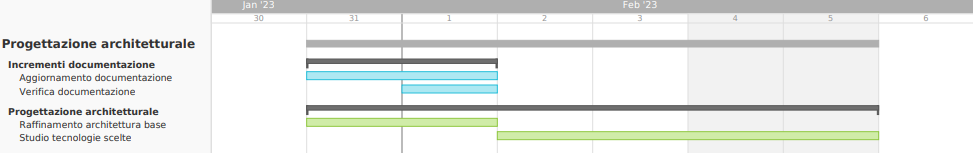
\includegraphics[width=\textwidth]{img/4_progettazione.png}
\caption{Progettazione architetturale}
\end{figure}

\subsection{Progettazione di dettaglio e Codifica}
Questa fase ha lo scopo di avviare le attività riguardanti la progettazione di dettaglio del sistema e la codifica del prodotto.
In particolare, la codifica si svolgerà in base alle norme di codifica stabilite nelle Norme di Progetto e avrà tra gli obiettivi anche l’assicurarsi di scrivere codice facilmente verificabile per facilitare il lavoro della fase successiva. Questo in quanto l'efficacia dei metodi di verifica\textsubscript{G} è strettamente legata alla qualità di strutturazione del codice. In questo modo non sarà necessario dipendere solo dalla verifica\textsubscript{G} retrospettiva, il cui costo cresce con l'avanzare della fase di codifica.

\subsubsection{Periodo}
La fase di progettazione di dettaglio e Codifica si svolgerà dal 20/02/2023 fino al 02/04/2023.

\subsubsection{Precondizioni}\:
\begin{itemize}
    \item È stata conclusa la progettazione architetturale ad alto livello.
\end{itemize}

\subsubsection{Postcondizioni}\:
\begin{itemize}
    \item Conclusione della progettazione di dettaglio;
    \item Conclusione di codifica e verifica\textsubscript{G}.
\end{itemize}

\subsubsection{Attività}\:
\begin{itemize}
    \item \textbf{Incremento e verifica\textsubscript{G} dei documenti}: A seconda delle necessità, il gruppo si occupa di aggiornare la documentazione prodotta in precedenza;
    \item \textbf{Product baseline}: Vengono studiati in dettaglio i design pattern\textsubscript{G} da utilizzare e prodotti relativi diagrammi;
        \subitem \textbf{Definizione delle unità software\textsubscript{G} che comporranno il prodotto}: Il prodotto viene suddiviso in unità, ciascuna delle quali potrà essere realizzata da un singolo programmatore;
    \item \textbf{Codifica}: Utilizzando il \textit{PoC\textsubscript{G}} prodotto in precedenza come base, viene prodotto il restante codice; la codifica avverrà utilizzando un approccio incrementale, per cui ogni incremento sarà costituito dalla codifica di un determinato caso d’uso e produrrà valore aggiunto;
        \subitem \textbf{verifica\textsubscript{G}}: Il codice prodotto viene continuamente verificato, tramite tecniche di analisi statica e dinamica - quest’attività prepara il successo della fase di validazione\textsubscript{G};
    \item \textbf{Stesura dell’allegato tecnico}: Viene prodotto il documento che descrive le caratteristiche architetturali del prodotto;
    \item \textbf{Stesura del manuale per la manutenzione del prodotto}: Viene prodotto il manuale per la manutenzione e le estensioni future del prodotto;
    \item \textbf{Stesura del manuale utente}: Viene prodotto il manuale contenente le istruzioni di utilizzo del prodotto;
    \item \textbf{Preparazione della presentazione per la revisione \textit{PB}}: Il gruppo si dedica alla preparazione dell’esposizione degli obiettivi raggiunti.
\end{itemize}

\subsubsection{Ruoli attivi}
Durante la fase di progettazione di dettaglio e Codifica saranno necessari i seguenti ruoli:
\begin{itemize}
	\item Responsabile;
    \item Amministratore;
    \item Progettista;
    \item Programmatore;
    \item Verificatore.
\end{itemize}

\subsubsection{Suddivisione temporale}
La fase di progettazione di dettaglio e Codifica è stata suddivisa in tre periodi distinti, analizzati di seguito. La milestone\textsubscript{G} individuata è rappresentata dalla revisione \textit{PB}.

\subsubsubsection{Primo periodo}\:
\begin{itemize}
    \item Dal 20/02/2023 al 26/02/2023.
\end{itemize}
Nel primo periodo viene conclusa la progettazione di dettaglio e iniziata la stesura dell’Allegato tecnico: a questo punto ogni attività di codifica può essere avviata in base alle scelte architetturali fatte dal gruppo.

\subsubsubsection{Secondo periodo}\begin{itemize}
    \item Dal 27/02/2023 al 26/03/2023.
\end{itemize}
Nel secondo periodo il gruppo si dedica alle attività di codifica e verifica\textsubscript{G}. Ad ogni sprint\textsubscript{G} review\textsubscript{G} vengono analizzati i risultati raggiunti e studiato un piano di azione per lo sprint\textsubscript{G} successivo, in modo da mantenere un’elevata capacità di rispondere alle eventuali problematiche riscontrate. Al termine di questo periodo il MVP\textsubscript{G} è pronto per la revisione \textit{PB}.

\subsubsubsection{Terzo periodo}\:
\begin{itemize}
    \item Dal 27/03/2023 al 02/04/2023.
\end{itemize}
Nel terzo periodo vengono redatti i manuali per la manutenzione e l’utilizzo del prodotto, e viene preparata la presentazione per la revisione \textit{PB}.

\subsubsection{Diagramma di Gantt\textsubscript{G} - Progettazione di dettaglio e Codifica}

\begin{figure}[H]
\centering
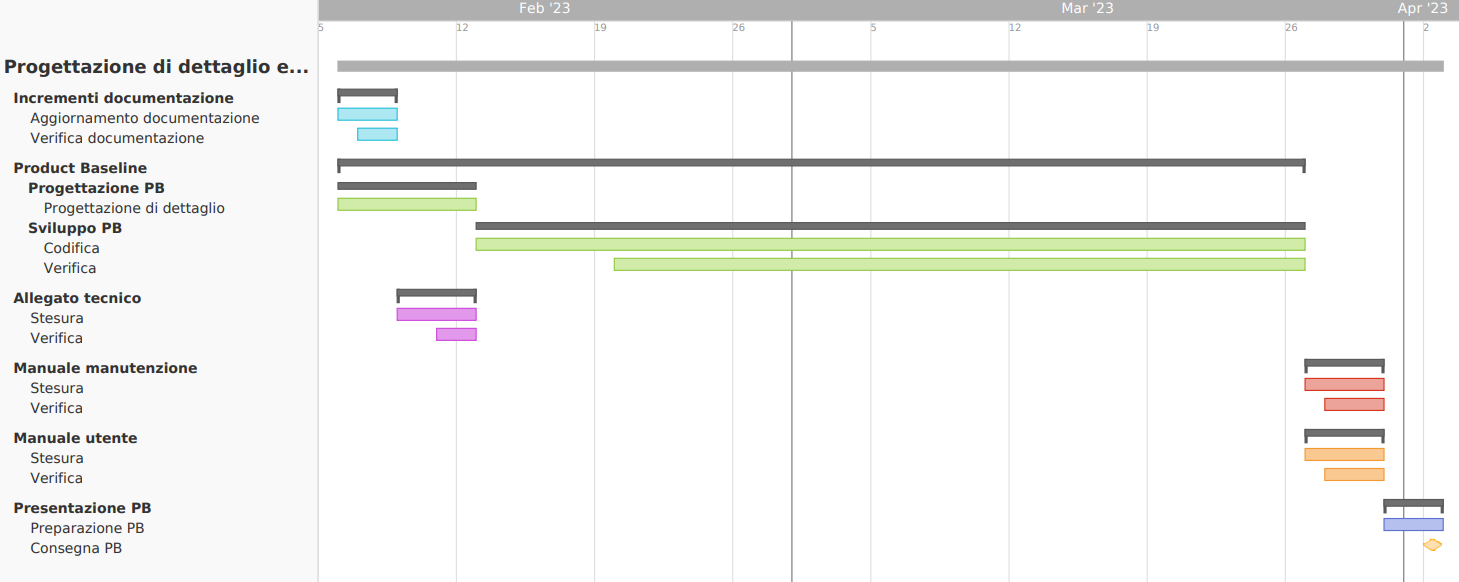
\includegraphics[width=\textwidth]{img/4_codifica.png}
\caption{Progettazione di dettaglio e Codifica}
\end{figure}

\newpage
\subsection{Validazione\textsubscript{G} e Collaudo}
In questo periodo vengono effettuati i controlli per garantire che i prodotti necessari alle varie revisioni soddisfino le attese degli stakeholder. Il progetto si concluderà con una verifica\textsubscript{G} del comportamento del sistema completo rispetto ai requisiti\textsubscript{G} stabiliti in precedenza, in presenza del committente.

\subsubsection{Periodo}
Il periodo di validazione e collaudo avrà i suoi sprint assegnati alle fasi di progetto precedenti alle revisioni RTB, PB e CA. Sarà quindi un periodo che sarà presente in varie fasi del progetto e i vari sprint che lo comporranno svolgeranno attività di validazione e collaudo dei vari prodotti nelle diverse fasi del progetto.

\subsubsection{Ruoli attivi}
Durante la fase di validazione\textsubscript{G} e Collaudo saranno necessari i seguenti ruoli:
\begin{itemize}
	\item Responsabile;
	\item Amministratore;
	\item Programmatore;
	\item Verificatore.
\end{itemize}

\subsubsection{Sprint VI}
\subsubsubsection{Scopo}
Lo scopo del sesto sprint è quello di validare e collaudare i documenti necessari alla revisione RTB e il Proof of Concept sviluppato. A seguito della validazione il \textit{Re} dovrà dare il consenso al rilascio dei prodotti.
\subsubsubsection{Durata}
Questo sprint si svolgerà a seguito del completamento del PoC e dei vari documenti necessari alla revisione RTB. Inizierà il 13/02/2023 e terminerà prima della revisione, pianificata per il 24/02/2023.

\subsubsubsection{Precondizioni}\:
\begin{itemize}
	\item È stato completato lo sviluppo del PoC;
	\item Sono stati completati tutti i documenti per la revisione RTB.
\end{itemize}

\subsubsubsection{Postcondizioni}\:
\begin{itemize}
	\item PoC e documenti sono stati rilasciati in versione 1.0.0;
	\item Completata la presentazione per la revisione RTB.
\end{itemize}

\subsubsubsection{Attività}\:
\begin{itemize}
	\item \textbf{Validazione documenti}: Vengono validati tutti i documenti per l'RTB. Il \textit{Re} si occuperà del loro rilascio.
	\item \textbf{Validazione e collaudo del PoC}: Il PoC sviluppato dovrà essere testato e collaudato per accertarsi che sia coerente con le aspettative e che gli obiettivi prefissati siano stati raggiunti;
	\item \textbf{Preparazione presentazione RTB}: Viene preparata la presentazione per la revisione RTB;
	\item \textbf{Lettera di candidatura}: Viene scritta la lettera che dichiara l'impegno del gruppo a candidarsi alla revisione RTB.
\end{itemize}








\subsubsection{Precondizioni}\:
\begin{itemize}
    \item È stata conclusa la progettazione di dettaglio;
    \item Sono state concluse la codifica e la verifica\textsubscript{G}.
\end{itemize}

\subsubsection{Postcondizioni}\:
\begin{itemize}
    \item Produzione dei test necessari;
    \item Esecuzione e superamento di tutti i test.
\end{itemize}

\subsubsection{Attività}\:
\begin{itemize}
    \item \textbf{Incremento e verifica\textsubscript{G} dei documenti}: a seconda delle necessità, il gruppo si occupa di aggiornare la documentazione prodotta in precedenza;
    \item \textbf{validazione\textsubscript{G} e Collaudo}: viene verificato che il prodotto finale soddisfi i requisiti\textsubscript{G} stabiliti tenendo in considerazione anche gli obiettivi di qualità definiti nel Piano di Qualifica;
    \item \textbf{Preparazione della presentazione per la revisione \textit{CA}}: il gruppo si dedica alla preparazione dell’esposizione degli obiettivi raggiunti.
\end{itemize}



\subsubsection{Suddivisione temporale}
La fase di validazione\textsubscript{G} e Collaudo è stata suddivisa in due periodi distinti, analizzati di seguito. La milestone\textsubscript{G} individuata è rappresentata dalla revisione \textit{CA}.

\subsubsubsection{Primo periodo}\:
\begin{itemize}
    \item Dal 03/04/2023 fino al 24/04/2023.
\end{itemize}
Nel primo periodo vengono effettuati tutti i test necessari; è possibile che in questo periodo sia necessario un incremento del codice in base ai risultati dei test.

\subsubsubsection{Secondo periodo}\:
\begin{itemize}
    \item Dal 25/04/2023 fino al 30/04/2023.
\end{itemize}
Nel secondo periodo il gruppo si dedica alla preparazione della presentazione per la revisione \textit{CA}.

\subsubsection{Diagramma di Gantt\textsubscript{G} - validazione\textsubscript{G} e Collaudo}

\begin{figure}[H]
\centering
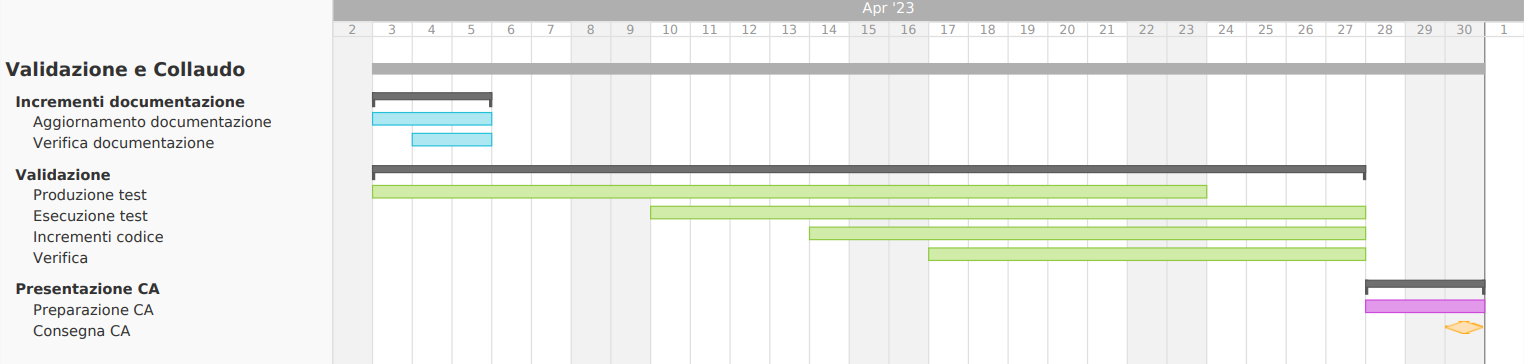
\includegraphics[width=\textwidth]{img/4_collaudo.png}
\caption{validazione\textsubscript{G} e Collaudo}
\end{figure}

